
Se desea realizar un despliegue del proyecto, de forma que los modelos de predicción sean accesibles mediante una interfaz web. Específicamente, se plantea que cualquier usuario 
pueda seleccionar una de las estaciones de GRAFCAN, y a partir de la misma, que la aplicación web devuelva la predicción de alguna de las variables meteorológicas en las próximas horas. 
Se decide arbitrariamente acotar la predicción a la variable de temperatura y a las próximas 6 horas.

Se realiza una interfaz web sencilla como front-end, y un back-end que maneje la carga de trabajo de predicción. Las predicciones se ejecutan de forma asíncrona 
para no bloquear la experiencia del usuario y permitir un cierto nivel de paralelismo.

\section{Front-end}
Tras valorar distintas opciones, se decide emplear React como framework para el front-end. Se elige por su facilidad de uso y la gran cantidad de librerías que existen para este.
Se emplea Typescript para la codificación, al ser una alternativa más robusta a Javascript, y que permite detectar errores de forma más sencilla.

Se crea una aplicación de una sola página (Single Page Application) que permite al usuario buscar y seleccionar una estación de GRAFCAN. Una vez seleccionada,
se envía una petición al back-end para obtener la predicción.

Las características de la aplicación son las siguientes:
\begin{itemize}
    \item \textbf{Selector de estaciones}: Permite al usuario seleccionar una estación de GRAFCAN. Se agrupan las estaciones por ubicación para facilitar la búsqueda.
    \item \textbf{Visualización de sensores}: Una vez seleccionada la estación, se muestran los sensores disponibles en la misma. 
    \item \textbf{Indicadores visuales de estado de la predicción}: Se utilizan indicadores visuales para mostrar el estado de la predicción. Estos indicadores permiten al usuario saber si la predicción está en curso, ha fallado o se ha completado con éxito.
\end{itemize}


Para el desarrollo de la aplicación es necesario crear una serie de elementos denominados \char`\"componentes". Estos componentes son bloques de código que 
permiten crear una interfaz de usuario modular y reutilizable. En este caso, se crean, entre otros:
\begin{itemize}
    \item \textbf{Dashboard}: Componente principal de la aplicación. Se encarga de gestionar el estado de la aplicación y de renderizar los demás componentes.
    \item \textbf{Selector de estaciones}: permite al usuario seleccionar una estación de GRAFCAN, ordenadas por ubicación geográfica.
    \item \textbf{Gráficas de sensor}: Se utilizan para mostrar los datos históricos de la estación seleccionada. 
    \item \textbf{Estado de predicción}: Indicadores permiten al usuario saber si la predicción está en curso, ha fallado o se ha completado con éxito.
    \item \textbf{Información de estación}: Muestra información detallada de la estación seleccionada, incluyendo los sensores disponibles y su estado.
\end{itemize}

La figura \ref{frontend_loading} muestra un ejemplo de la interfaz web mientras se recuperan los datos de una estación, la figura 
\ref{frontend_loaded} contiene el resultado y en \ref{frontend_prediction} se muestra el resultado de una predicción.

\begin{figure}[H]
    \centering
    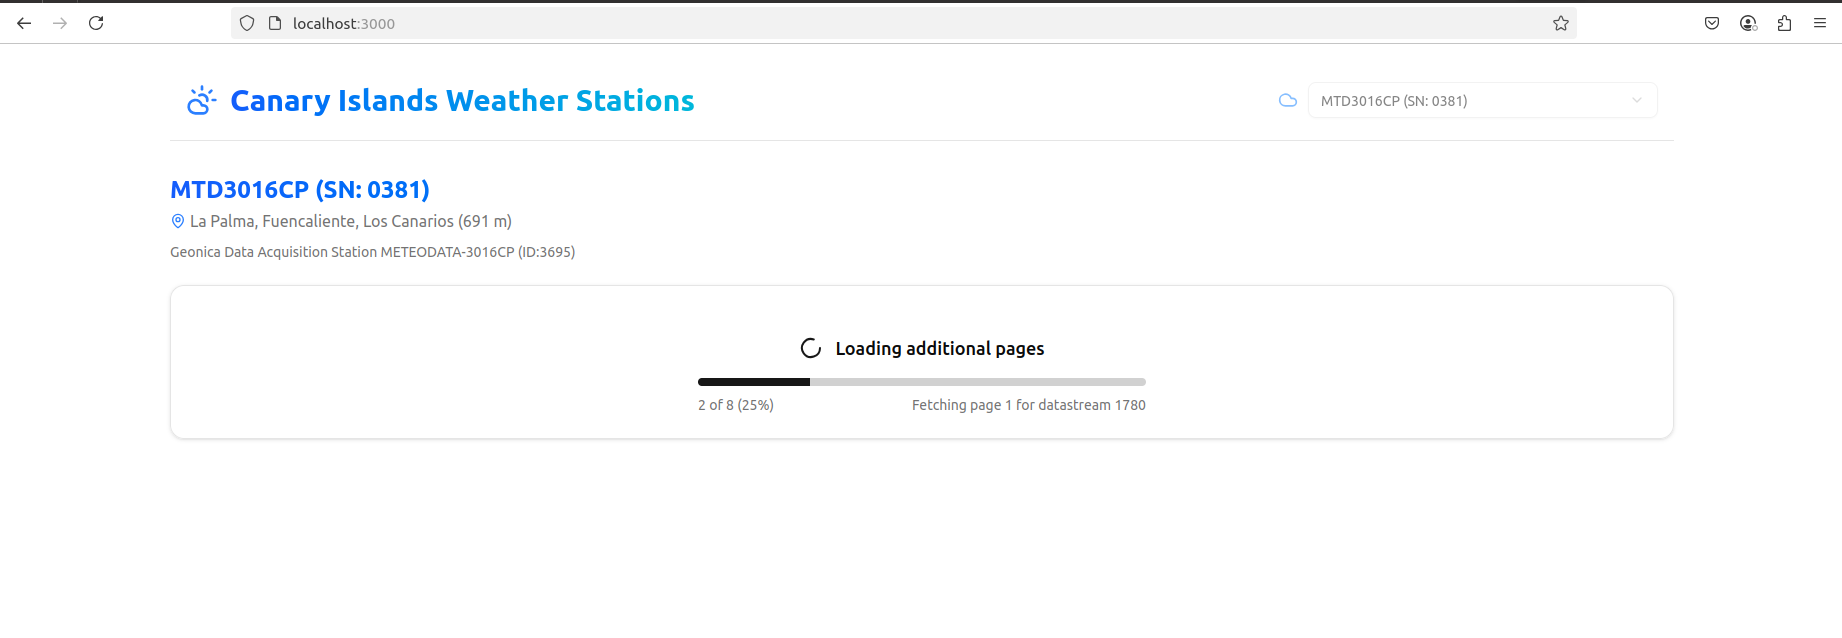
\includegraphics[width=0.9\textwidth]{images/frontend_loading.png}
    \caption{Interfaz web. Carga de datos de una estación}
    \label{frontend_loading}
\end{figure}

\begin{figure}[H]
    \centering
    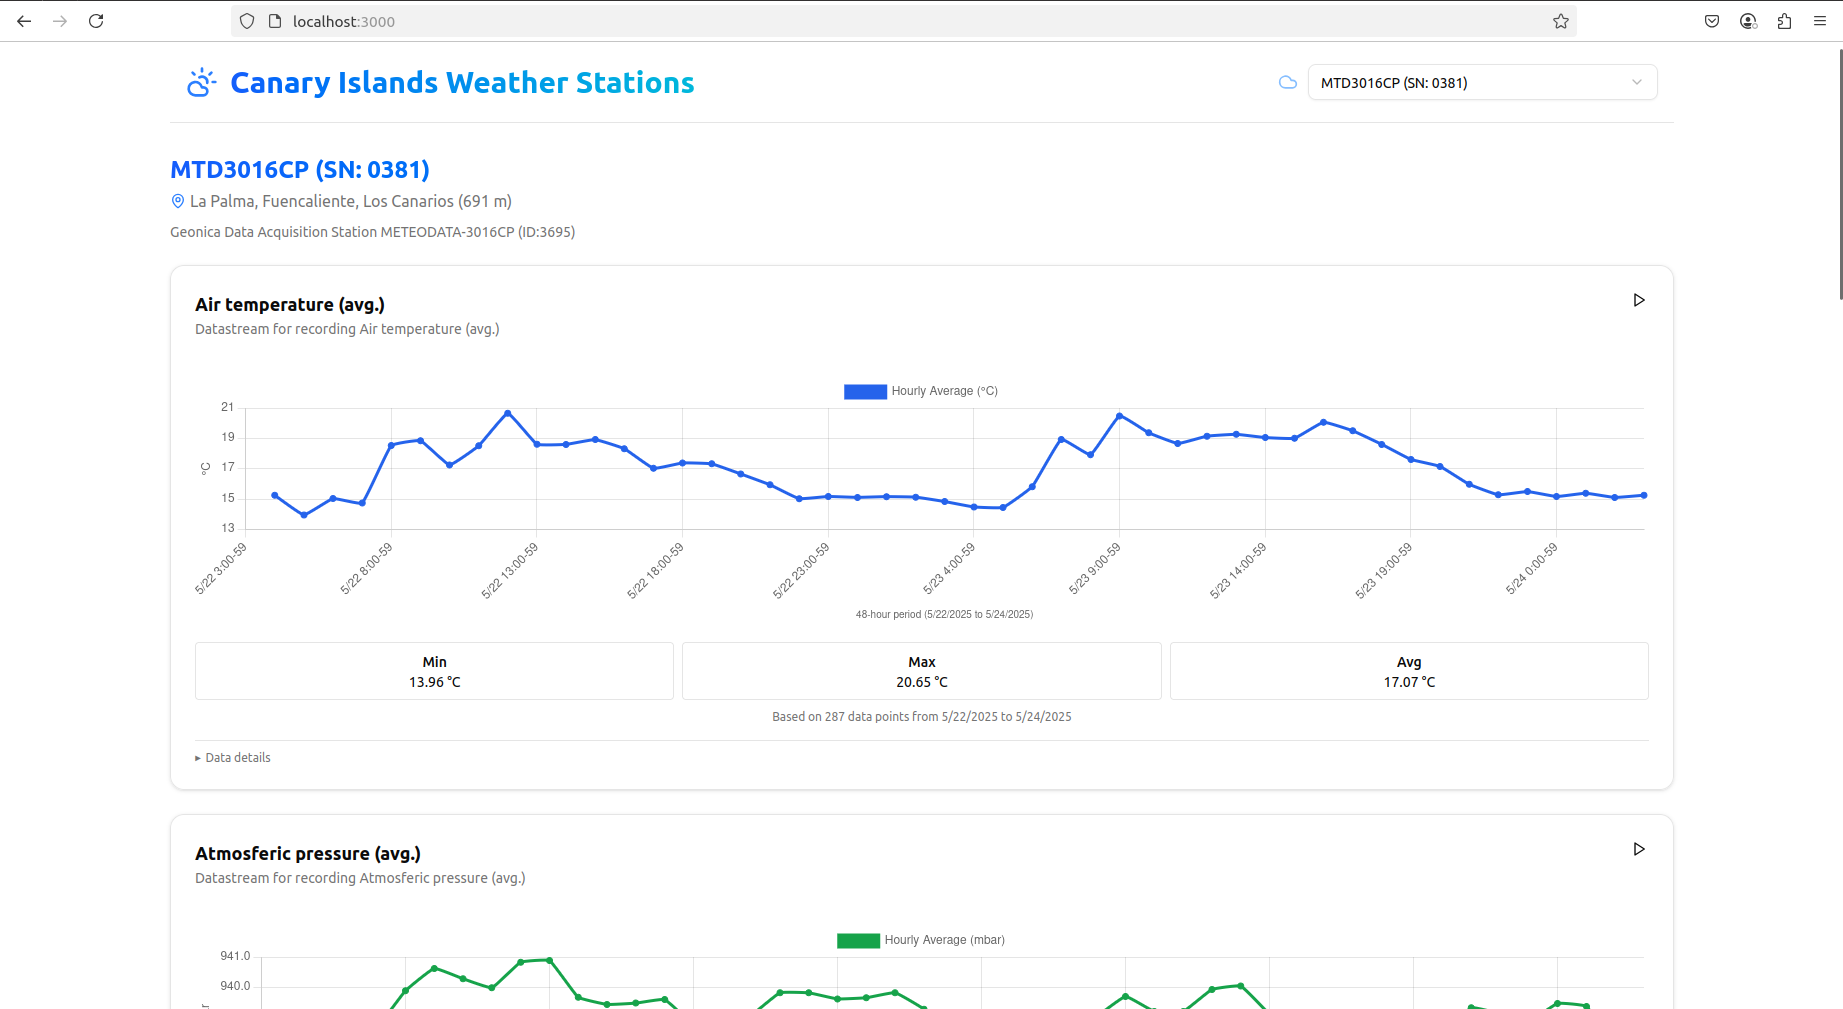
\includegraphics[width=0.9\textwidth]{images/frontend_loaded.png}
    \caption{Interfaz web. Gráfica con datos de una estación}
    \label{frontend_loaded}
\end{figure}

\begin{figure}[H]
    \centering
    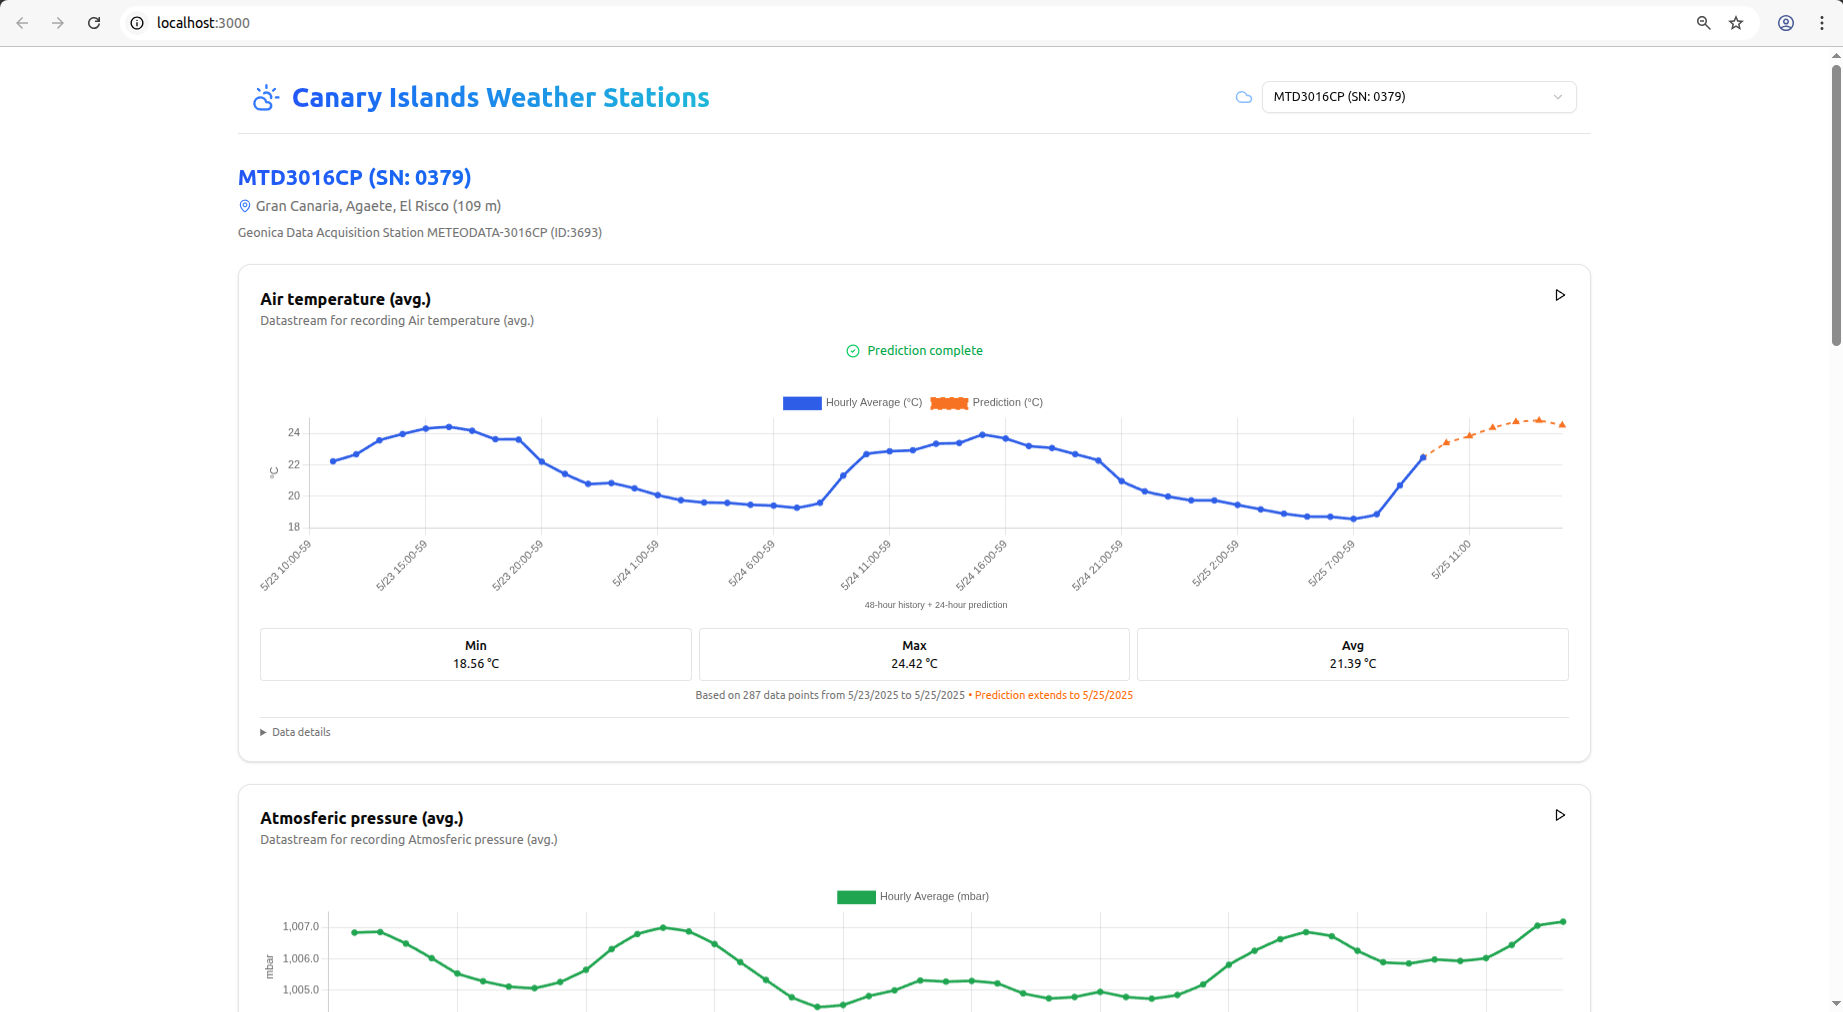
\includegraphics[width=0.9\textwidth]{images/frontend_prediction_6.png}
    \caption{Interfaz web. Resultado de una predicción}
    \label{frontend_prediction}
\end{figure}


\section{Back-end}

\begin{itemize}
    \item \textbf{FastAPI}: Se trata de un framework web para construir APIs en Python, que facilita crear servicios RESTful con alto rendimiento. Se emplea para gestionar las peticiones de predicción.
    \item \textbf{Worker Celery}: Como nodo trabajador se emplea Celery, una biblioteca de Python para ejecutar tareas asíncronas y distribuir trabajos en segundo plano, ideal para procesar tareas largas o programadas sin bloquear la aplicación principal. 
    Se utiliza como sistema de tareas asíncronas para evitar bloquear el servidor web durante la ejecución de las predicciones. El worker carga el modelo LSTM previamente entrenado al iniciarse, utilizando los pesos almacenados localmente. 
    \item \textbf{Redis}: Se utiliza como broker de tareas para Celery. Permite almacenar y gestionar las tareas encoladas, facilitando la comunicación entre el servidor web y los workers.
\end{itemize}

Esta arquitectura, que se muestra en la figura \ref{deploy_scheme}, facilita el despliegue, escalabilidad y mantenimiento del sistema, permitiendo además la ejecución paralela de múltiples workers para atender una mayor carga de solicitudes.
\begin{figure}[H]
    \centering
    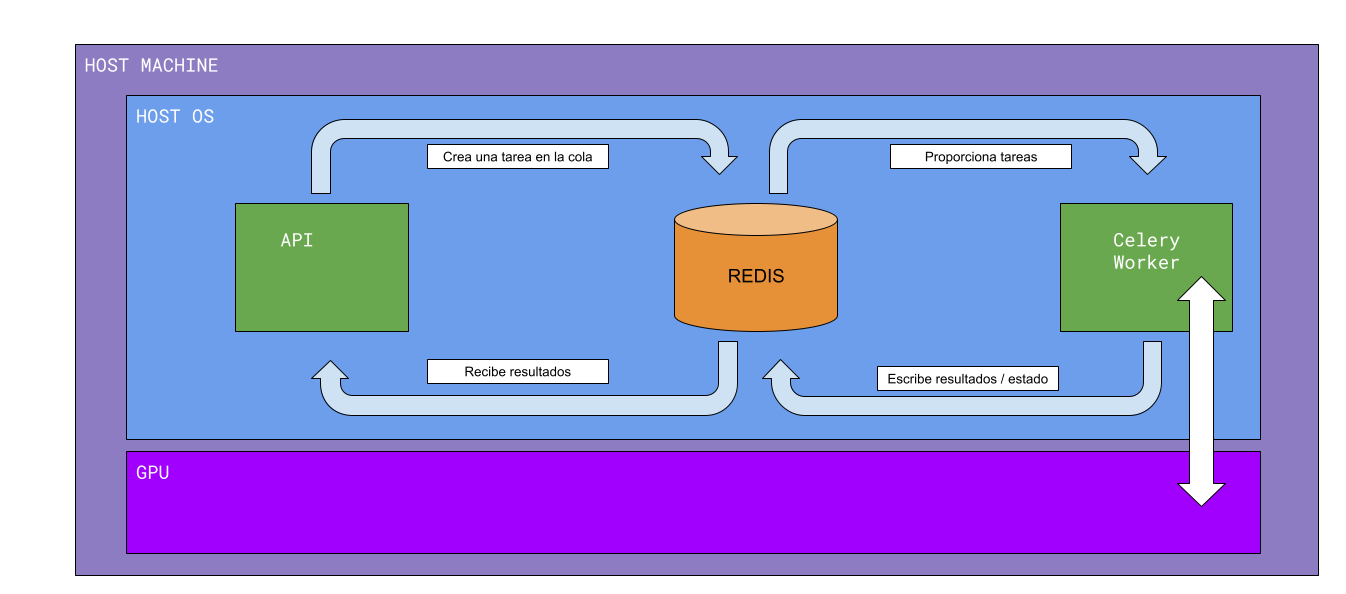
\includegraphics[width=0.9\textwidth]{images/esquema_despliegue.png}
    \caption{Esquema de la lógica del despliegue}
    \label{deploy_scheme}
\end{figure}

La API es responsable de validar y transformar los datos de entrada, preparar la estructura requerida por el modelo de predicción y coordinar la ejecución de las tareas de inferencia mediante Celery.

Los endpoints disponibles en la API son:

\begin{itemize}
    \item \textbf{POST $/$predict}:  recibe datos estructurados correspondientes a observaciones recientes de una estación. Estos datos se procesan para generar un tensor con forma [1, T, F], donde T representa el número de intervalos temporales considerados y F = 7 corresponde a las características de entrada (cuatro variables temporales codificadas mediante funciones seno y coseno para capturar patrones cíclicos diarios y anuales, y tres variables provenientes de sensores). A continuación, la solicitud es encolada como una tarea en Celery para su procesamiento.
    \item \textbf{GET $/$predict$/${job\_id}}: permite consultar el estado de la tarea asociada al identificador job\_id. En caso de que la predicción ya esté disponible, devuelve el resultado generado.
\end{itemize}
El procesamiento interno del back-end incluye la extracción de características temporales relevantes y la conversión de los datos a tensores NumPy que alimentan el modelo de predicción.


El flujo general de una petición de predicción es el siguiente:

\begin{itemize}
    \item El usuario selecciona una estación de GRAFCAN y un sensor específico en la interfaz web.
    \item El front-end recopila las observaciones de los últimos 48 intervalos horarios y envía esta información al back-end mediante el endpoint POST /predict.
    \item El back-end valida y transforma los datos, encolando la tarea en Celery.
    \item El worker procesa la tarea, ejecutando el modelo LSTM para obtener la predicción.
    \item El front-end consulta periódicamente el estado y resultado de la tarea mediante el endpoint GET /predict/{job\_id}.
    \item  Finalmente, el resultado se presenta visualmente, superponiéndose a las gráficas de las observaciones originales del sensor.
\end{itemize}

